% @Author: soheilred
% @Date:   2018-10-28 01:10:54
% @Last Modified by:   soheilred
% @Last Modified time: 2018-10-29 12:51:04
\documentclass{beamer}

\let\val\undefined
\usepackage{pgf}
\usepackage{pgfplots}
\usepackage{tikz}
\usepackage{booktabs}
\usepackage{natbib}
\usepackage{framed}
\usepackage{longtable}
\usepackage{bigdelim,multirow}
\usepackage{amsmath}
\usepackage{amsthm}
\usepackage{mathtools}


\usetikzlibrary{arrows,automata,backgrounds,positioning,decorations,intersections,matrix}

% *** Styles ***
\setbeamertemplate{navigation symbols}{}
\usecolortheme{dolphin}
%\usecolortheme{rose}
\setbeamercovered{transparent}
\usefonttheme{professionalfonts}
%\usefonttheme[onlymath]{serif}

% 
\addtobeamertemplate{navigation symbols}{}{%
    \usebeamerfont{footline} %
    \usebeamercolor[fg]{footline}%
    \hspace{1em}%
    \insertframenumber/\inserttotalframenumber
}

\DeclarePairedDelimiter{\norm}{\lVert}{\rVert}
\DeclarePairedDelimiter\abs{\lvert}{\rvert}%


% \setlist[itemize,1]{label=$\times$}
% \setlist[itemize,2]{label=$\checkmark$}
% \setlist[itemize,3]{label=$\diamond$}
% \setlist[itemize,4]{label=$\bullet$}


% *** Colors ***
\newcommand{\tc}[2]{\textcolor{#1}{#2}}
\newcommand{\tcb}[1]{\tc{blue}{#1}}
\newcommand{\tcr}[1]{\tc{red}{#1}}
\newcommand{\tcg}[1]{\tc{green}{#1}}

\def\checkmark{\tikz\fill[scale=0.4](0,.35) -- (.25,0) -- (1,.7) -- (.25,.15) -- cycle;} 

\newcommand{\Ex}{\mathbb{E}}
%\newcommand{\Pr}{\mathbb{P}}
\DeclareMathOperator{\Var}{Var}

\definecolor{varcolor}{RGB}{132,23,49}
\newcommand{\varname}[1]{\textcolor{varcolor}{\mathsf{#1}}}

\title{Reinforcement learning with automatic basis construction
based on isometric feature mapping}
\author{Z. Huang et al. \\ \textbf{Journal}: Information Sciences \\ \textbf{IF}: 4.305}
\date{}

\begin{document}
\begin{frame}
	\maketitle

\end{frame}
%=====================================%
\begin{frame}
	\frametitle{Background}
	\begin{itemize}
		\item Value function approximation has always been a big issue in RL
		\item In small problems \textbf{tabular representation} is enough. But, as the problem grows bigger, representing the $V(s), Q(s,a), P(s,a), R(s)$ becomes drastically hard
		\item We are looking for some ways to represent $Q(s,a)$ (or $V(s)$) in a more compressed format
		\[
			Q_{\abs{\mathcal{S}} \abs{\mathcal{M}}*1}(s,a) = \Phi w = \sum_{i = 1}^l \phi_i(s,a) w_i
		\] 
	
	\end{itemize}

\end{frame}
%=====================================%
%=====================================%

\begin{frame}
	\frametitle{Background}
	\begin{itemize}
		\item Finding good basis functions is crucial to the success of our solution
		\item Some options:
		\begin{itemize}
			\item Linear
			\item Polynomials
			\item Splines
			\item RBFs
			\item Fourier transforms
			\item Laplacian analysis
		\end{itemize}
		\item They need to be engineered!
		\item Can we automate the process?
	\end{itemize}
\end{frame}
%=====================================%
%=====================================%

\begin{frame}
	\frametitle{Problem Definition}
	\begin{itemize}
		\item Big MDPs, impossible to represent MDP with P and R in a regular way
		\item \tcg{We have:} a set of samples (trials or episodes)
		\item \tcg{We want:}
		\[
			\vec{\phi} = [ \phi_1(x), \phi_2(x), ... ,\phi_l(x)]
		\]
		where
		\[
			\tilde{V}(\mathcal{X}) = \vec{\phi}^T (\mathcal{X}) \vec{W}
		\]
		\[
			\mathcal{X} = \{ x_1, x_2, ... , x_n \}
		\]
		\item This process is called \emph{Learning Basis Functions}
		\item Given $\phi$s we can solve our MDP using standard solutions (LSPI, ALP,...) 
	\end{itemize}
\end{frame}
%=====================================%
%=====================================%

\begin{frame}
	\frametitle{Characteristics of the Solution}
	\begin{itemize}
		\item Mapping $X$ to $\Phi$
		\item Isometric feature mapping (IFM)
		\item Preserves geodesic distance\footnotemark[1] in the neighborhood graph for input and output
	\end{itemize}
	\begin{center}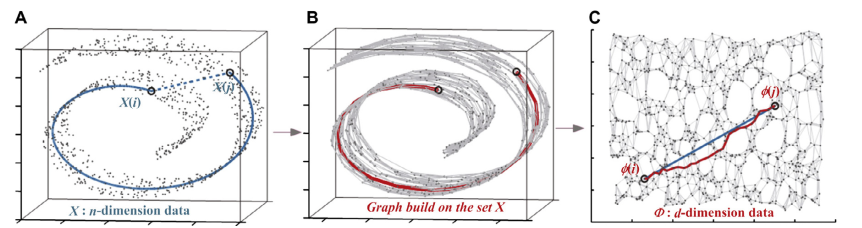
\includegraphics[width=\linewidth]{3.png}\end{center}	
	\footnotetext[1]{the distance between two vertices in a graph or the number of edges in a shortest path}
\end{frame}
%=====================================%
%=====================================%

\begin{frame}
	\frametitle{Basis Learning Process}
	Three steps:
	\begin{enumerate}
		\item Determine neighbor points (K-nearest neighbors is used)
		\item Geodesic distances ($d_{\mathcal{X}}(i,j)$) are estimated using shortest path
		\item A multidimensional scaling method is applied to analyze the graph distance matrix
	\end{enumerate}
\end{frame}
%=====================================%
%=====================================%

\begin{frame}
	\frametitle{IFM Algorithm}
	\begin{center}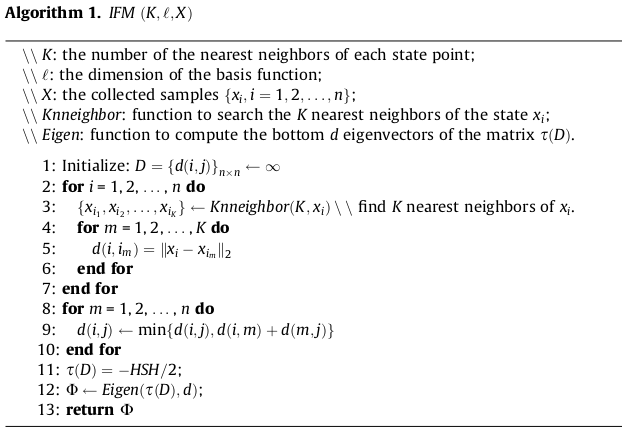
\includegraphics[width=\linewidth]{algo1.png}\end{center}	
	\footnotetext[1]{$S_{ij} = D_{ij}^2$ and $H_{ij} = \delta_{ij} - 1/N$}
	\footnotetext[2]{KNN has $\mathcal{O}(Knl)$ time complexity}
\end{frame}
%=====================================%
%=====================================%

\begin{frame}
	\frametitle{IFM-API}
	\begin{itemize}
		\item Sample Collection: Only a subset of samples are used to construct basis functions
		\begin{itemize}
		    \item[$\times$] Trajectory-based Sub-sampling
		    \item[\checkmark] Clustering-based Sub-sampling
		\end{itemize}
		\item Basis Learning based on isometric feature mapping
		\item Obtain basis functions corresponding to the whole state spaces based on the known basis functions in $X_s$
		\item At the end, they combined IFM with LSPI
	\end{itemize}
\end{frame}
%=====================================%


%=====================================%

\begin{frame}
	\begin{center}
		\Huge Thank You!
	\end{center}
\end{frame}
%=====================================%

% \begin{frame}
	% \frametitle{Background}
% 	\begin{itemize}
% 		\item 
% 	\end{itemize}
% \end{frame}


\end{document}
